\documentclass[12pt]{article}

\usepackage[total={6.5in,8.75in}, top=2.4cm, left=2.4cm]{geometry}
\usepackage{lineno}
\usepackage{amsmath}
%\usepackage{amssymb}    % used for symbols in figure legends
\usepackage{graphicx}
\usepackage[round,colon,authoryear]{natbib}

\usepackage{bm}
\usepackage{float}
\usepackage{amsmath}
\usepackage{amsfonts}
\usepackage{hyperref}
\usepackage{verbatim}
\usepackage{soul}
\usepackage{color}
\usepackage{setspace}

\bibliographystyle{ecology} % kluwer, plos-natbib, pnas-natbib


%\title{Ecological Distance in Spatial Capture-Recapture Models}
\title{Spatial Capture-Recapture Models for
Jointly Estimating Population Density and
Landscape Connectivity}

\begin{small}
\author{
{\bf J. Andrew Royle}, {\bf Richard B. Chandler},
{\bf Kimberly D. Gazenski} \\
USGS Patuxent Wildlife Research Center, Laurel MD \\ \\
{\bf Tabitha A. Graves}\footnote{
Current Address:
Colorado State University,
Warner College of Natural Resources,
201 JVK Wagar. 
Fort Collins, CO 80523
}
 \\
Northern Arizona University, Flagstaff AZ \\ \\
}
\end{small}


\begin{document}

\maketitle

\date


\linenumbers


\begin{spacing}{1.8}

\begin{flushleft}
{\em \bf Abstract}
Population density and landscape connectivity are key determinants of
population viability, yet no methods exist for
simultaneously estimating density and connectivity parameters.
Recently-developed spatial capture-recapture (SCR) models
provide a framework for estimating density of animal populations,
but thus far have not been used to study connectivity.  Rather, all
applications of SCR models have used encounter probability models
based on the Euclidean distance between traps and animal activity
centers, which implies that home ranges are stationary and
symmetric, and unaffected by landscape %or habitat
structure. In this paper we devise encounter probability models based
on ``ecological distance'', i.e., the least-cost path between
traps and activity centers, which is a function of both Euclidean
distance and animal movement behavior in %heterogeneous
resistant landscapes. We
integrate least-cost path models into a likelihood-based estimation
scheme for spatial capture-recapture models in order to estimate
population density and parameters of the least-cost encounter
probability model.  Therefore, it is possible to make explicit
inferences about animal density, distribution, and landscape
connectivity as it relates to animal movement from standard
capture-recapture data.  Furthermore, a simulation study demonstrated
that ignoring landscape connectivity can result in negatively biased density
estimators under the naive SCR model. % can be substantially
%biased when home ranges are not symmetric.

{\em \bf Key words:} animal movement, ecological distance, landscape connectivity,
least-cost path, resistance surface, spatial capture-recapture

\end{flushleft}



\section{Introduction}

Assessing the impacts of habitat fragmentation and habitat loss on
population density and landscape connectivity
are high priorities in applied ecological research.
Landscape connectivity is defined as the
degree to which landscape structure impedes or facilitates movement
\citep{tischendorf_fahrig:2000} and is widely recognized to be an
important component of population viability
\citep{with_crist:1995}. Although much theory has
been developed to predict the effects of decreasing
connectivity, few empirical studies have been conducted to test these
predictions due to the paucity of formal methods for estimating connectivity
parameters \citep{cushman_etal:2010}. Instead, ecologists often rely on expert opinion or
\textit{ad hoc} methods of specifying connectivity values, even in
important applied settings
\citep{adriaensen_etal:2003,beier_etal:2008,zeller_etal:2012}. In addition, no
methods are available for simultaneously estimating population density and
connectivity parameters, in spite of theory
predicting interacting effects of density and connectivity on
population viability \citep{tischendorf_etal:2005,cushman_etal:2010}.

%Before introducing our model for density and connectivity, we note
%that the simple objective of estimating population density of mobile
%organisms is challenging in and of itself because movement can
%invalidate assumptions of standard models, such
%distance sampling, which require spatially-independent observations.
Spatial capture-recapture (SCR) models are a relatively new class of
models allowing for inference about both population density and
movement %designed for estimating population density of mobile organisms
\citep{efford:2004,borchers_efford:2008, royle_young:2008, efford_etal:2009ecol,
  royle_etal:2009ecol}. While SCR models are a relatively recent innovation,
their use is already becoming widespread \citep{efford_etal:2009ecol,
  gardner_etal:2010jwm, gardner_etal:2010ecol,kery_etal:2010,
  gopalaswamy_etal:2012ecol, foster_harmsen:2012} because they resolve
critical problems with ordinary non-spatial capture-recapture
methods such as ill-defined area sampled and heterogeneity in
encounter probability due to the juxtaposition of individuals with
traps. Furthermore,
 all capture-recapture studies produce auxiliary spatial
information and therefore SCR models are widely applicable.


In spite of their utility for estimating population density, SCR
methods are still in their infancy, and so far, every application
has implicitly assumed that animals have isotropic home
ranges and that movement is unaffected by landscape
structure. Specifically, existing SCR models assume that %capture
encounter
probability is a simple function of the Euclidean distance between an
individual's activity center (e.g. its home range or territory center)
and the trap location.
While these simple encounter probability models will often
be sufficient for some purposes, especially in small data sets,
%sometimes developing more complex models of the capture %detection
%process as it relates to space usage of individuals will be useful.
animals may not judge distance in terms of Euclidean distance but,
rather, according to the quality of local habitat, %landscape connectivity,
perceived mortality risk, and other considerations that facilitate or
impede movement. Because %capture
encounter probability and the distance
metric upon which it is based represent outcomes of individual
movements about their home range, it is desirable to relax the
Euclidean distance assumption of SCR models such that
% offer a means of evaluating %ecologists might have explicit
hypotheses about landscape connectivity
%how landscape structure affects movement
can be evaluated.



In this paper we develop models for encounter probability based on
alternative distance metrics that account for
%ecological considerations---
connectivity---which, in keeping with the conventions in the
ecological literature, we will call ``ecological distance''. In
particular, we adopt a cost-weighted distance metric to define the
{\it least-cost path}, which is 
used widely in landscape ecology for modeling resistance to movement
and gene flow \citep{adriaensen_etal:2003}. In the
%%%%%%%%%%,manel_etal:2003,mcrae_etal:2008}. In the
context of SCR models we can use this as the basis for defining the 
distance between traps and individual's activity centers. In this way
we can explicitly model the effects of %accommodate
landscape structure on movement.
%and account for how animals use space in SCR models.
We develop a likelihood-based inference framework that allows
estimation of the parameters of the cost function
%for SCR model parameters using
%this new distance metric when the ecological distance function is
%known.  We show that the maximum likelihood estimates (MLEs) are approximately unbiased in moderate
%sample sizes, as expected, but also that the misspecified model based
%on Euclidean distance can produce substantial bias in estimates of $N$
%and hence density.  Further, we extend the model to allow for likelihood
%estimation of parameters of the cost function,
so that direct inference about density and connectivity can be made
from capture-recapture data without subjective prescription
of resistance or cost surfaces.


\section{Spatial Capture-Recapture}

The basic idea of SCR is to express encounter probability %of individuals
as a function of the distance between an individual's 
activity center, say ${\bf s}$, and a trap location, say ${\bf x}$ \citep{borchers_efford:2008}. The
definition of an activity will be context-specific, but often it will
be the center of an individual's home range, or more generally, the
spatial average of an individual's locations during some time
period. SCR methods regard the activity centers as latent variables
following some spatial point process, such as the homogeneous
model ${\bf s} \sim \mbox{Uniform}({\cal
  S})$ where ${\cal S}$ is a spatial region (the ``state-space'' of
${\bf s}$)
%, or a model in which covariates might affect the spatial
%distribution of individuals
\citep{royle_young:2008}.
The state-space ${\cal S}$
defines the potential locations for any activity center ${\bf s}$, e.g.,
a polygon defining available habitat or range of the species under study.

%In these models ${\bf s}_{i}$ is regarded as a latent variable and
%conventional methods of statistical inference either based on marginal
%likelihood \citep{borchers_efford:2008} or Bayesian analysis by MCMC
%\citep{royle_young:2008}.

A number of distinct encounter %observation
models have been proposed for
spatial capture-recapture situations \citep{borchers_efford:2008,
  royle_etal:2009ecol, efford_etal:2009ecol}, including Poisson,
multinomial or binomial %observation
models.
%The most appropriate
%observation model for a dataset depends upon the the sampling method.
%For example, when animals are physically captured and retained in
%traps, then the multinomial model is appropriate because it does not
%allow for an individual to be captured in multiple traps during a
%single occasion.
Here we focus on the binomial model in which we
suppose that $J$ traps at locations ${\bf x}_{j}$ are operated for $K$
occasions (e.g., nights), although our development of ecological distance
models is directly applicable to other observation models without any
further technical considerations. The binomial model is most directly
relevant to devices such as hair snares
\citep{woods_etal:1999,gardner_etal:2010jwm} or scent sticks
\citep{kery_etal:2010} for which individuals can only be encountered
at most once in a trap per observation occasion.

The observations are individual- and trap-specific counts $y_{ij}$
which are binomial with sample size $K$ and probabilities
$p_{ij}$. The vector of trap-specific counts for individual $i$,
 ${\bf y}_{i} = (y_{i1},\ldots,y_{iJ})$ is its {\it encounter history}.
A standard encounter probability model
\citep{borchers_efford:2008} is the Gaussian model in which

\begin{equation}
log(p_{ij})= \alpha_{0} + \alpha_{1} d({\bf x}_{j}, {\bf s}_{i})^{2}
\label{eq.encounter}
\end{equation}
or, equivalently,
$p_{ij} = \lambda_{0} exp(-  d({\bf x}_{j}, {\bf s}_{i})^{2}
/(2\sigma^{2}) )$
where $\alpha_{0} = log(\lambda_{0})$ and $\alpha_{1} =
-1/(2\sigma^2)$ and $d({\bf x}_{j}, {\bf s}_{i})$ is the Euclidean
distance between trap $j$ and activity center $i$.


Although alternative detection models are often used, all are
functions of Euclidean distance and so we do not consider them
further. The distance metric we develop subsequently can be
used in conjunction with any other detection model.  In all previous
applications of SCR models the Euclidean distance has been
used, i.e., $ d({\bf x}_{j}, {\bf s}_{i}) = ||{\bf x}_{j} - {\bf
  s}_{i}||$, and the parameters $\alpha_0$ and $\alpha_1$ have been
estimated using standard methods (likelihood or Bayesian).

The critical assumption that motivates our work is that the Euclidean
distance metric is unaffected by habitat or landscape structure, and
it implies that the space used by individuals is stationary (invariant
to translation) and symmetric
which may be unreasonable in some applications.  For example, if the
common detection model based on a bivariate normal probability
distribution function is used, then the implied space usage by {\it
  all} individuals, no matter their location in space or local habitat
conditions, is symmetric with circular contours of usage intensity
(density contours of the probability density).  Subsequently we provide an extension
of this class of SCR models that accommodates alternative distance
metrics that explicitly incorporate information about the landscape so
that a unit of distance is variable depending on identified
covariates. Thus, where an individual lives on the landscape, and
the state of the surrounding landscape, will determine the nature
of its usage of space. In particular, we suggest distance metrics that
imply irregular, asymmetric and non-stationary home ranges of
individuals. An example of this is shown in Fig. \ref{fig.homeranges}
which shows home ranges of 4 individuals for a specific landscape,
described below.



\section{Cost-Weighted Distance}

We adopt the use of a cost-weighted distance metric here which defines
the distance between locations by accumulating cell-specific costs
determined under a cost function defined by the user.  The idea of
cost-weighted distance to characterize animal use of landscapes is
widely used in landscape ecology for modeling connectivity, movement
and gene flow \citep{beier_etal:2008}. As is customary for reasons of
computational tractability we consider a discrete landscape defined by
cells 
of some prescribed resolution. The distance between any two
locations ${\bf x}$ and ${\bf x}'$ can be represented by a sequence of
line segments connecting neighboring cells say ${\bf l}_{1},{\bf
  l}_{2},\ldots,{\bf l}_{m}$. Then the total cost-weighted distance between
${\bf x}$ and ${\bf x}'$ is

\begin{equation}
 d({\bf x},{\bf x}')
  =  \sum_{i=1}^{m-1} cost({\bf l}_{i},{\bf l}_{i+1})||{\bf l}_{i} - {\bf l}_{i+1}||
\label{eq.costweighted}
\end{equation}

{\flushleft
where } $cost({\bf l}_{i},{\bf l}_{i+1})$ is the user-defined cost function
to move
from cell ${\bf l}_{i}$ to neighboring cell ${\bf l}_{i+1}$ in the sequence.
Given the ``cost'' of each cell, it is a simple matter to compute the
cost-weighted distance between any two cells, along {\it any} path,
by accumulating the incremental  cost-weighted 
distances.
In the context of
SCR models (and, more generally, landscape
connectivity) we are concerned with the {\it minimum} cost-weighted
distance, that of the {\it least-cost path}, between any two locations which
we will denote by $d_{lcp}$, which is
the
sequence ${\bf l}_{1},{\bf l}_{2},\ldots,{\bf l}_{m}$ that minimizes
Eq. \ref{eq.costweighted}. That is,

\begin{equation}
 d_{lcp}({\bf x},{\bf x}')
  =  min_{{\bf l}_{1},\ldots,{\bf l}_{m}}  \sum_{i=1}^{m-1} cost({\bf l}_{i},{\bf l}_{i+1})||{\bf l}_{i} - {\bf l}_{i+1}||
\label{eq.lcp}
\end{equation}

{\flushleft
 Least-cost} path can be calculated in
 many geographic information systems and other software packages,
including the {\bf R} package \mbox{\tt
  gdistance} \citep{vanetten:2011}.


The key ecological aspect of least-cost path modeling is the
development
of models for cell-specific cost (also called {\it resistance} in the
landscape ecology literature).
In this paper we model cost as a log-linear function of covariates
defined on every cell, i.e., $z({\bf x})$ is the value of some
covariate at location ${\bf x}$.
%{\flushleft This} is interpreted as cost of moving {\it through} a
%pixel but, in practice,
Then, we model cost of
moving from a cell ${\bf x}$ to one of its neighbors, say ${\bf
  x}'$, by the weighted average

\begin{equation}
 log(cost({\bf x},{\bf x}'))=  \alpha_{2} \frac{z({\bf x})+z({\bf x}')}{2}
\label{eq.cost}
\end{equation}

{\flushleft
where $\alpha_{2}$ is the resistance parameter to be estimated.} Thus, if $\alpha_{2} = 0$ then substituting $cost({\bf x},{\bf x}')
=exp(0) = 1$ into
Eq. \ref{eq.lcp} will produce the ordinary Euclidean distance
between points.

In practical applications, variables that influence the cost of moving
across the landscape include highways
\citep[e.g.,][]{epps_etal:2005}, elevation \citep{cushman_etal:2006},
 snow cover
\citep{schwartz_etal:2009}, distance to escape terrain
\citep{shirk_etal:2010}, or range limitations
\citep{mcrae_beier:2007}.  Together multiple environmental variables
create a resistance surface, which forms the linchpin of all
connectivity planning \citep{spear_etal:2010}.
 Although $\alpha_{2}$ is never known in practice,
conservation biologists design linkages that require this resistance
value as input \citep[see][and articles cited
therein]{beier_etal:2008}.
Therefore, investigators often choose a value for $\alpha_{2}$
based on
expert opinion \citep{beier_etal:2008}, although recently researchers
have begun to define costs based on resource selection functions,
animal movement \citep{tracy:2006, fortin_etal:2005}, or genetic
distance data \citep{gerlach_musolf:2000,
schwartz_etal:2009}. Our paper represents the first formal approach
to estimating landscape resistance parameters from capture-recapture data.
%The published
%methods require many assumptions and these estimates have not been
%integrated with capture-recapture methods, nor have parameters been
%formally estimated using capture-recapture data.

To formalize the use of cost-weighted distance in SCR models, we
substitute Eq. \ref{eq.lcp} in the expression for encounter
probability (Eq. \ref{eq.encounter}) and maximize the resulting
likelihood (see {\it Maximum Likelihood Estimation}), including for estimating the
parameter $\alpha_{2}$. An example of computing cost-weighted distance
in {\bf R} for a simple landscape is given in Appendix 1.


\subsection{Non-stationarity of home range structure}

When distance is defined by the cost-weighted distance metric given
by Eq. \ref{eq.lcp} then individual space-usage varies
spatially in response to the landscape covariate(s) used in the
distance metric. For example, we use the two landscapes shown in
Fig. \ref{ecoldist.fig.raster100}
in 
our simulation study below. The landscape shown in the right panel, with
distance
metric defined by Eq. \ref{eq.lcp}, produces home ranges such
as those shown in Fig. \ref{fig.homeranges}. Later we simulate data
under the model that produces these home ranges and fit spatial
capture-recapture models to evaluate the efficacy of likelihood
estimation under this model.




\section{Maximum likelihood estimation}
\label{sec.mle}

Here we outline a standard method of parameter estimation based on
marginal likelihood. That is, the likelihood in which the latent
variables ${\bf s}$ are removed by integration \citep{borchers_efford:2008}.
The individual- and trap-specific observations have a binomial
distribution conditional on the latent variable ${\bf s}_{i}$:

\begin{equation}
  y_{ij}| {\bf s}_{i} \sim \mbox{Binomial}(K, p_{\bm \alpha}(d_{lcp}({\bf x}_{j},{\bf s}_{i};\alpha_{2}); \alpha_{0}, \alpha_{1})
\label{mle.eq.cond-on-s}
\end{equation}

{\flushleft where} we have indicated the dependence of $p$ on the parameters
${\bm \alpha} =(\alpha_{0},\alpha_{1},\alpha_{2})$, and also $d_{lcp}$ which
itself depends on $\alpha_{2}$, and the latent variable ${\bf s}$.
%The parameters
%${\bm \alpha}$ include whatever parameters are involved in the
%cost-weighted distance function, i.e., at least $\alpha_{2}$ from
%Eq. \ref{eq.cost}.
For the random effect we have ${\bf s}_{i} \sim  \mbox{Uniform}({\cal
  S})$.
The joint distribution of the data for individual $i$ is the product
of $J$ binomial terms (i.e., contributions from each of $J$ traps):
$[{\bf y}_{i} | {\bf s}_{i} , {\bm \alpha}] = 
  \prod_{j=1}^{J} \mbox{Binomial}(K, p_{\bm \alpha}({\bf x}_{j},{\bf s}_{i}) )$.
%This assumes independence of capture in each trap.
%Conditional on
%${\bf s}_{i}$ this is reasonable in most applications in our view.
 The so-called marginal likelihood is computed by removing
${\bf s}_{i}$, by integration,  from the conditional-on-${\bf s}$
likelihood and regarding the {\it marginal} distribution of the data
as the likelihood. That
is, we compute:

\[
  [{\bf y}_{i}|{\bm \alpha}] =
\int_{{\cal S}}  [ {\bf y}_{i} |{\bf s}_{i},{\bm \alpha}] g({\bf s}_{i}) d{\bf s}_{i}
\]

{\flushleft where}, under the uniformity assumption, we have
$g({\bf s}) = 1/||{\cal S}||$.
The joint likelihood for all $N$ individuals,
is the product of $N$ such terms:

\[
{\cal L}({\bm \alpha} | {\bf y}_{1},{\bf y}_{2},\ldots, {\bf y}_{N}) 
= \prod_{i=1}^{N} [{\bf y}_{i}|{\bm \alpha}]
\]

Because $N$ is unknown, 
we have to accommodate the contribution of $N-n$ ``all-zero''
encounter histories (i.e., $y_{ij} = 0$ for all $j$). 
We include the number of such all-zero encounter histories as
an unknown parameter of the model, which we label $n_{0}$.  In
addition, we have to be sure to include a combinatorial term to
account for the fact that of the $n$ observed individuals there are
${N \choose n}$ ways to realize a sample of size $n$. The
combinatorial term involves the unknown $n_{0}$ and thus it must be
included in the likelihood.
Technical details for computing the likelihood and obtaining the MLEs
are given in Appendix 2 where we provide an ${\bf R}$ function
to evaluate the likelihood and obtain the MLEs.
A key practical detail is that the likelihood here is formulated in
terms of the parameter $N$, the population size for the landscape
defined by ${\cal S}$. Given ${\cal S}$, density
is
computed as $D({\cal S}) = N/||{\cal S}||$ where $\|\mathcal{S}\|$ is
the area of the state space. In our simulation study
below we report $N$ as the two are equivalent summaries of the data
set once ${\cal S}$ is defined.


%\section{Examples of SCR Models with Landscape Resistance}
\section{Examples}

In this section we provide examples that we think are typical of how
cost-weighted distance models can be used in real capture-recapture
problems.  We define a $20 \times 20$ cell landscape with
extent = $[0.5, 4.5] \times [0.5, 4.5]$.
%We define this landscape by
%a single covariate for determing the cost function, and we consider
%two specific covariates.
%purposes of our example, as a coarse landscape covariate, with pixels
%having some arbitrary scaling say, a $2 \times 2$ km resolution. Thus,
%the raster defines a landscape of $40 \times 40$ km and we suppose
We suppose that 16 camera traps are established at the integer coordinates
$(1,1), (1,2), \ldots, (4,4)$. We could think of this as a landscape
within which we're studying a population of ocelots, lynx or some
other species using camera traps.

For our analyses, cost is characterized by a single covariate
and we consider two specific cases. First is an increasing trend from
the NW to the SE (``systematic landscape''), where $z(x)$ is defined as
$z(x) = r(x) + c(x)$ where $r(x)$ and $c(x)$ are just the row and
column, respectively, of the landscape.  This might define something
related to distance from an urban area or a gradient in habitat
quality due to land use, or environmental conditions such as
temperature or precipitation gradients.  In the second case we make up
a covariate by generating a field of spatially correlated noise to
emulate fragmented habitat.
%a typical patchy habitat covariate (''patchy landscape'') such as
%tree or understory density.
The two covariates are shown in Fig. \ref{ecoldist.fig.raster100},
along with a sample realization of
$N=100$ individuals (left panel only).  For both covariates we use a
cost function in which transitions from cell ${\bf x}$ to ${\bf x}'$
is given by:

\[
 log(cost({\bf x},{\bf x}'))=  \alpha_2 \frac{z({\bf x}) + z({\bf x}')}{2}
\]

{\flushleft where} $\alpha_2 = 1$ for our simulation.


\subsection{Simulation study}

We devised a limited simulation study to evaluate three things: (1)
the general statistical performance of the density estimator under
this new model; (2) the effect of mis-specifying the model with a
normal Euclidean distance metric and (3) the statistical performance
of estimating the resistance parameter, $\alpha_{2}$.

We used population sizes of 100 and 200 individuals with activity
centers randomly distributed on the $20 \times 20$ landscape, and subjected them
to encounter by 16 traps arranged in a $4\times 4$ grid according to
the Euclidean distance metric. We fit 3 different models; (i) the
misspecified Euclidean distance model; (ii) the true data-generating
model with the cost {\it known} and (iii) the true
data-generating model but estimating the resistance parameter by
maximum likelihood.  We used the ``systematic'' and ``fragmented'' %``patchy''
covariates defined previously.

We simulated encounter data for the $N$ individuals using the Gaussian
encounter model with least-cost path distance metric:

\[
log(p_{ij})= \alpha_{0} + \alpha_{1} d_{lcp}({\bf x}_{j},{\bf
  s}_{i}; \alpha_{2})^{2}
\]

{\flushleft We } used here $\alpha_{0} = -2$ and $\alpha_{1} = 2$, the latter value
corresponding to $\sigma = 0.5$ of a stationary bivariate normal home
range model.  We varied the number of replicate samples $K=3,5,10$
(e.g., nights in a camera trapping study) to produce varying sample
sizes.  Because any simulation study is inherently arbitrary, we have
provided {\bf R} scripts for carrying out simulations in Appendix 2 so
that the interested reader can experiment with their own situations.




\subsection{Simulation Results}

For both landscapes and all simulation conditions (levels of $K$ and
$N$) the average sample sizes of individuals captured are given in
Appendix 4.  The simulation results for estimating $N$
for the prescribed state-space are given in Table 1.
For the fragmented %``patchy''
landscape we see extreme
bias in estimates of $N$ when the Euclidean distance is used. There is
moderate small sample bias of 3-5\% in the MLE of $N$ using the
least-cost path distance which becomes negligible as $K$ increases. For
$N=200$ the bias is on the order of 2\% for the lowest sample size
case ($K=3$) but negligible otherwise.  Interestingly, for the
landscape exhibiting systematic trend, there is a persistent bias
in the MLE of $N$ of 1-3\% even for the highest level of $K$. We were
initially surprised by this but, in fact, it results from
the state-space being small relative to the extent of the trap grid, and
sensitivity to a state-space that is too small is expected because the
support of the integrand is truncated. In the particular case of the
systematic landscape, we find that, on some edges of the landscape
where cost of movement is low, individuals use large areas of space,
and the fitted model is under-stating the apparent
heterogeneity in encounter probability for the prescribed landscape.  We
found that the issue is resolved when the traps are moved away from
the boundary (see Appendix 4).

The performance of estimating the resistance parameter $\alpha_{2}$ mirrors
the results for estimating $N$ for the prescribed area
(Appendix 4). In the fragmented %patchy
landscape where we don't expect a systematic gradient in space
usage around the edge of the state-space, we find
that $\alpha_{2}$ is estimated with
diminishing bias as the sample size increases, but with persistent
bias due to truncation of the likelihood for the systematic
landscape which, as with the MLE of $N$, is resolved by moving the
traps away from the edge of the prescribed landscape ${\cal S}$. Equivalently, in practice,
this could be resolved by expanding ${\cal S}$ away from the trap
locations so that all regions used by animals exposed to capture are
included in ${\cal S}$.



\section{Discussion}



Inferences about population density and landscape connectivity
%the structure of ecological distance
are fundamental to many problems in
applied and theoretical ecology such as the assessment of fragmentation
effects, corridor and reserve design, gene flow, and population viability
analysis.  Our  model allows
investigators to address these problems using non-invasively collected
capture-recapture data by evaluating the landscape
factors influencing movement. % of individuals.
%over the landscape from non-invasively collected capture-recapture data.
%Therefore spatial-capture recapture models based on ecological
%distance metrics might aid in corridor design and understanding other
%aspects of space usage and movement in animal populations.
%In this paper, we developed the first formal framework for inference
%about population density and landscape connectivity. To do so, we
Our approach involves replacing the ordinary Euclidean distance metric
in SCR models with %integrating ``ecological distance'', % into SCR
                   %models, where ecological distance is
an ``ecological distance'' metric defined as the minimum cost-weighted
distance (i.e., ``least-cost
path'') between points, and where ``cost'' is characterized by one or
more spatially explicit covariates that are believed to influence
movement. % or space-usage of individuals.
Unlike many previous efforts, we presented methods for estimating the
parameters of the cost function, thereby eliminating the need to
subjectively prescribe their value.




Animal movement is associated with various behaviors such as dispersal and
migration, which may operate over many spatial and temporal
scales. For simplicity, we considered movement around
fixed home range centers, and thus our model is most applicable to
short time intervals such as a single breeding season. %Understanding
Connectivity at this time scale is important because, for example,
it can determine which breeding individuals interact. When
interest lies in the effects of connectivity on more complex movement
behaviors such as dispersal, we expect that it
would be possible to extend our model to allow for movement of the
activity centers themselves. Specifically, we envision cost-weighted
distance functions that would describe the location of activity
centers at time $t$ as a function of their location at time $t-1$ and
the landscape structure surrounding the initial location
\citep{gardner_etal:2010ecol}. By adopting
this type of open population model, it might also be possible to study
the factors affecting dispersal propensity and survival during
dispersal. Several capture-recapture methods exist for modeling
dispersal
\citep{kendall_nichols:2004,fujiwara_etal:2006,ovaskainen_etal:2008},
but none
allows for estimation of density and landscape connectivity.



Our paper also has implications for existing SCR studies.
Not surprisingly, our simulation study demonstrated
(Tab. 1)
that the MLE of model parameters is
approximately unbiased in moderate sample sizes. Moreover, the effect
of ignoring ecological distance and using normal Euclidean distance in
the model for encounter probability, has the logical effect of causing
negative bias in estimates of $N$.  We expect this because the effect
is similar to failing to model heterogeneity, i.e., if we mis-specify
``model Mh'' with ``model M0''
\citep{otis_etal:1978} then we will expect to under-estimate $N$
\citep[][p. 193]{royle_dorazio:2008}. So
the effect of mis-specifying the ecological distance metric with a
standard homogeneous Euclidean distance has the same effect. As a
practical matter, it stands to reason that many previous applications
of SCR models based on homogeneous distance metrics have under-stated
density of the focal population.

Our approach to modeling landscape connectivity does not include an
explicit model of animal movement. That is, we cannot make inferences
about the precise location of movement paths taken between recapture
events or temporal decisions made by the animal as it moves about the
landscape. Rather, our model describes the probability that an animal
is captured at a trap based on the landscape context associated with
the trap and the animal's activity center. Equivalently, our model
describes the process by which animals use space, and thus could be
regarded as a model of resource selection. Although this is more
phenomenological than an explicit movement model, it is consistent
with the concepts of landscape connectivity and
resistance. Furthermore, it is possible that our model could be
expanded to accommodate telemetry data or other information if
movement behavior is of interest.

Some additional methodological extensions may be of general interest.
We adopted a standard approach to inference under our model based on
marginal likelihood but, in principle, Bayesian analysis does not pose
any unique challenges for this class of models, except that computing
the cost-weighted distance is computationally intensive and having to
do this at each iteration of an MCMC algorithm may be impractical. We
have used least-cost paths here to represent ecological distance
although other distance metrics could be used, including circuit
resistance distances \citep{mcrae:2006}. Instead of characterizing
cost with explicit covariates it might be possible to estimate the
``resistance surface'' as a latent field, much as \citet{wikle:2003}
did in the developing of models of species spread based on a diffusion
process. He defined the spatially-explicit rate of diffusion,
$\delta(x)$, as a Gaussian spatial process, and it was estimated from
the data.


Capture-recapture methods are one of the most common technique for studying
animal populations and, with new technologies such as camera trapping
and DNA sampling,
it is possible to conduct research on species that
previously could not be studied. Our modeling framework makes it
feasible to use basic capture-recapture data to study landscape
connectivity and density simultaneously.




\newpage


\bibliography{EDmanuscript-v3.bbl}


\end{spacing}



\clearpage

\newpage


\begin{table}[h!]
{\small
\caption{Simulation results for estimating population size $N$ for a
  prescribed landscape with
$N=100$ or $N=200$ and various levels of replication ($K$) chosen to affect the observed sample
size of individuals (see Appendix 1 for details). For each simulated data set, the SCR model was fitted with
standard Euclidean distance (``euclid''), least-cost path assuming the
resistance 
parameter $\alpha_2$ is known (``lcp/known''), or allowing it to
be estimated by maximum likelihood (``lcp/est'').
The summary statistics of the
sampling distribution reported are the mean, standard deviation
(``SD'') and quantiles (0.025, 0.50, 0.975).
}
{\bf Systematic trend landscape:} \\
\begin{tabular}{l|rrrrr|rrrrr}
         & \multicolumn{5}{c}{N=100   } & \multicolumn{5}{c}{N=200  }  \\
         &   mean &  SD  & 0.025 & 0.50 & 0.975  & mean  & SD   & 0.025 & 0.50  & 0.975 \\ \hline
K=3      &        &      &       &      &        &       &      &       &       &       \\
euclid   &   63.65& 12.62& 44.77 & 61.17&  90.98 & 126.68& 17.05&  98.93& 124.49& 168.26 \\
lcp/known&   99.28& 20.80& 68.83 & 97.55& 152.59 & 196.47& 27.39& 152.03& 192.96& 259.78\\
lcp/est  &  101.93& 21.68& 67.95 &101.56& 156.21 & 201.58& 28.14& 154.96& 200.15& 263.20\\
K=5      &        &      &       &      &        &       &      &       &       &        \\
euclid   &  64.60 & 7.11 & 51.52 & 63.86&  77.33 & 130.02& 10.25& 113.48& 128.96& 151.32\\
lcp/known&  95.96 &11.64 & 74.21 & 96.16& 117.65 & 193.04& 17.13& 166.84& 191.88& 226.16\\
lcp/est  &  98.94 &12.97 & 74.68 & 99.00& 123.88 & 198.80& 19.60& 166.87& 197.97& 239.46\\
K=10     &        &      &       &      &        &       &      &       &       &       \\
euclid   &  69.24 & 4.83 & 59.37 & 69.47&  79.18 & 139.83&  7.62& 125.65& 139.65& 154.82\\
lcp/known&  94.46 & 7.04 & 81.45 & 94.04& 108.83 & 190.47& 11.55& 170.49& 189.74& 213.19\\
lcp/est  &  97.53 & 8.18 & 82.02 & 97.62& 113.16 & 195.19& 13.28& 171.63& 194.58& 217.96\\ \hline
\end{tabular}
\\
{\bf Fragmented landscape: } \\ %Patchy "random" landscape: } \\
\begin{tabular}{l|rrrrrrrrrr}
         & \multicolumn{5}{c}{N=100  } & \multicolumn{5}{c}{N=200   }  \\
         &   mean &  SD  & 0.025 & 0.50  & 0.975  & mean  & SD   & 0.025 & 0.50  & 0.975 \\ \hline
K=3      &        &      &       &       &        &       &      &       &       &       \\
euclid   &  78.68 & 18.12& 49.40 & 76.34 & 125.47 & 154.34& 33.74& 107.00& 146.34& 221.43\\
lcp/known& 109.09 & 27.52& 69.50 &104.86 & 183.72 & 207.18& 46.53& 143.31& 198.42& 315.89\\
lcp/est  & 110.96 & 28.65& 69.55 &106.98 & 181.84 & 208.77& 49.29& 141.68& 197.89& 325.77\\
K=5      &        &      &       &       &        &       &      &       &       &        \\
euclid   &  77.85 & 11.55& 59.17 & 77.44 & 101.14 & 153.39& 15.57& 129.31& 149.54& 185.38\\
lcp/known& 103.57 & 15.83& 78.15 &100.58 & 137.48 & 201.57& 21.25& 165.94& 199.95& 243.26\\
lcp/est  & 104.44 & 15.79& 78.38 &101.47 & 139.55 & 200.91& 20.78& 164.42& 200.47& 246.46\\
K=10     &        &      &       &       &        &       &      &       &       &       \\
euclid   &  78.01 & 5.26 & 68.00 & 77.96 & 87.81  & 156.27&  8.51& 142.17& 156.05& 174.55\\
lcp/known&  99.84 & 7.09 & 86.86 & 99.84 & 114.11 & 198.64& 11.04& 181.43& 197.62& 220.45\\
lcp/est  & 100.42 & 7.56 & 86.72 &100.34 & 115.47 & 198.45& 11.44& 180.06& 198.04& 219.52\\ \hline
\end{tabular}
}
\label{tab.results1}
\end{table}





\begin{comment}

\begin{table}[ht]
\centering
\caption{
Mean of sampling distribution of the resistance parameter 
$\alpha_{2}$ for the different simulation
conditions.
}
\begin{tabular}{l|rrrr}
 & \multicolumn{2}{c}{Patchy} & \multicolumn{2}{c}{Systematic} \\
    & N=100 &  N=200  &   N=100 &  N=200  \\ \hline
K=3 &   1.05&    1.03 &     1.17 & 1.14 \\
K=5 &   1.02&    1.01 &     1.12 &1.12 \\
K=10&   1.01&    1.00 &     1.10 &1.08 \\
\end{tabular}
\label{tab.results2}
\end{table}



\end{comment}






\newpage

{\flushleft \bf LIST OF FIGURES:}

\vspace{.2in}


{\flushleft \bf
Figure 1:}
Typical home ranges for 4 individuals in the fragmented landscape. %based on the ``patchy'' cost surface.
The black dot indicates the home
  range center and the cells around each home range center are shaded
according to the probability of encounter, if a trap were located in
that cell.



\vspace{.2in}


{\flushleft \bf Figure 2:}
Two landscape covariates used for simulations. The left image
represents a systematic trend that might mimic distance from a habitat
feature. The right image is a patchy covariate generated by spatially
correlated noise. A hypothetical
  realization of $N=100$ activity centers is superimposed on the left
  (black dots),
along with 16 trap locations (red dots).


\newpage


% Figures


\begin{figure}
\begin{center}
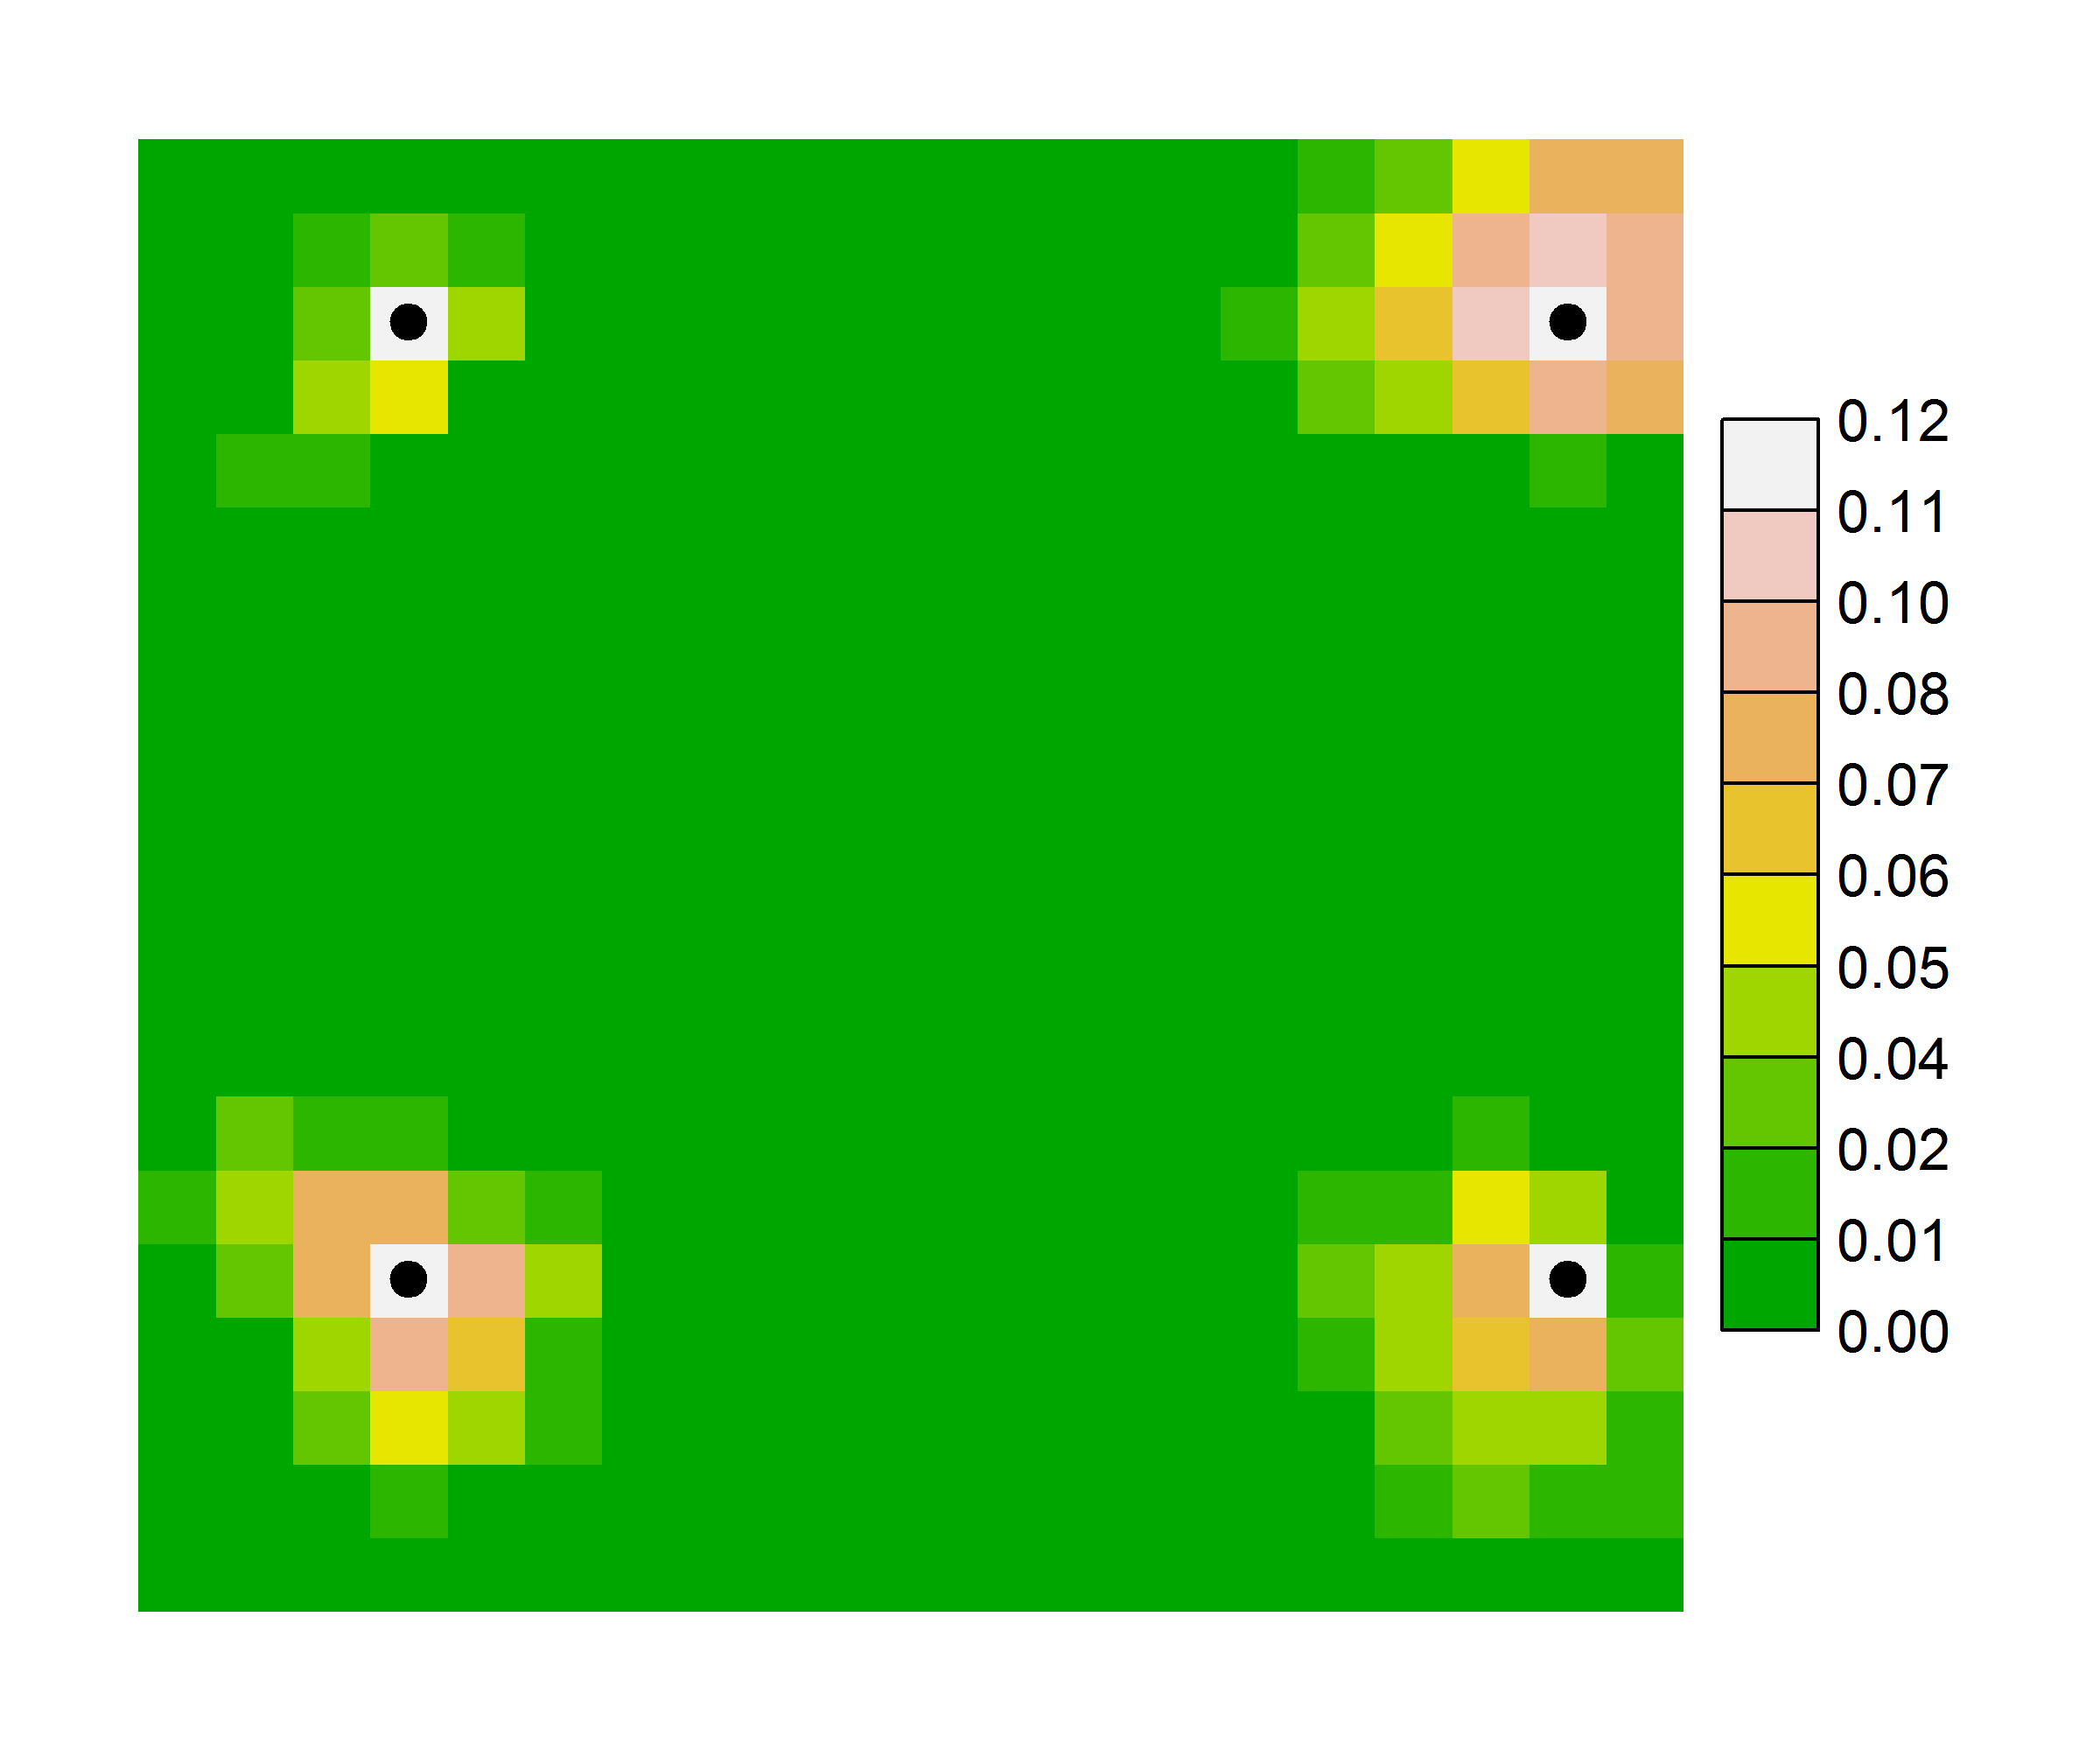
\includegraphics[height=5in,width=6in]{home_rangesv2}
\end{center}
\caption{
Typical home ranges for 4 individuals in the fragmented landscape. %based on the ``patchy'' cost surface.
The black dot indicates the home
  range center and the cells around each home range center are shaded
according to the probability of encounter, if a trap were located in
that cell.
}
\label{fig.homeranges}
\end{figure}

\clearpage
\newpage


\begin{figure}
\begin{tabular}{cc}
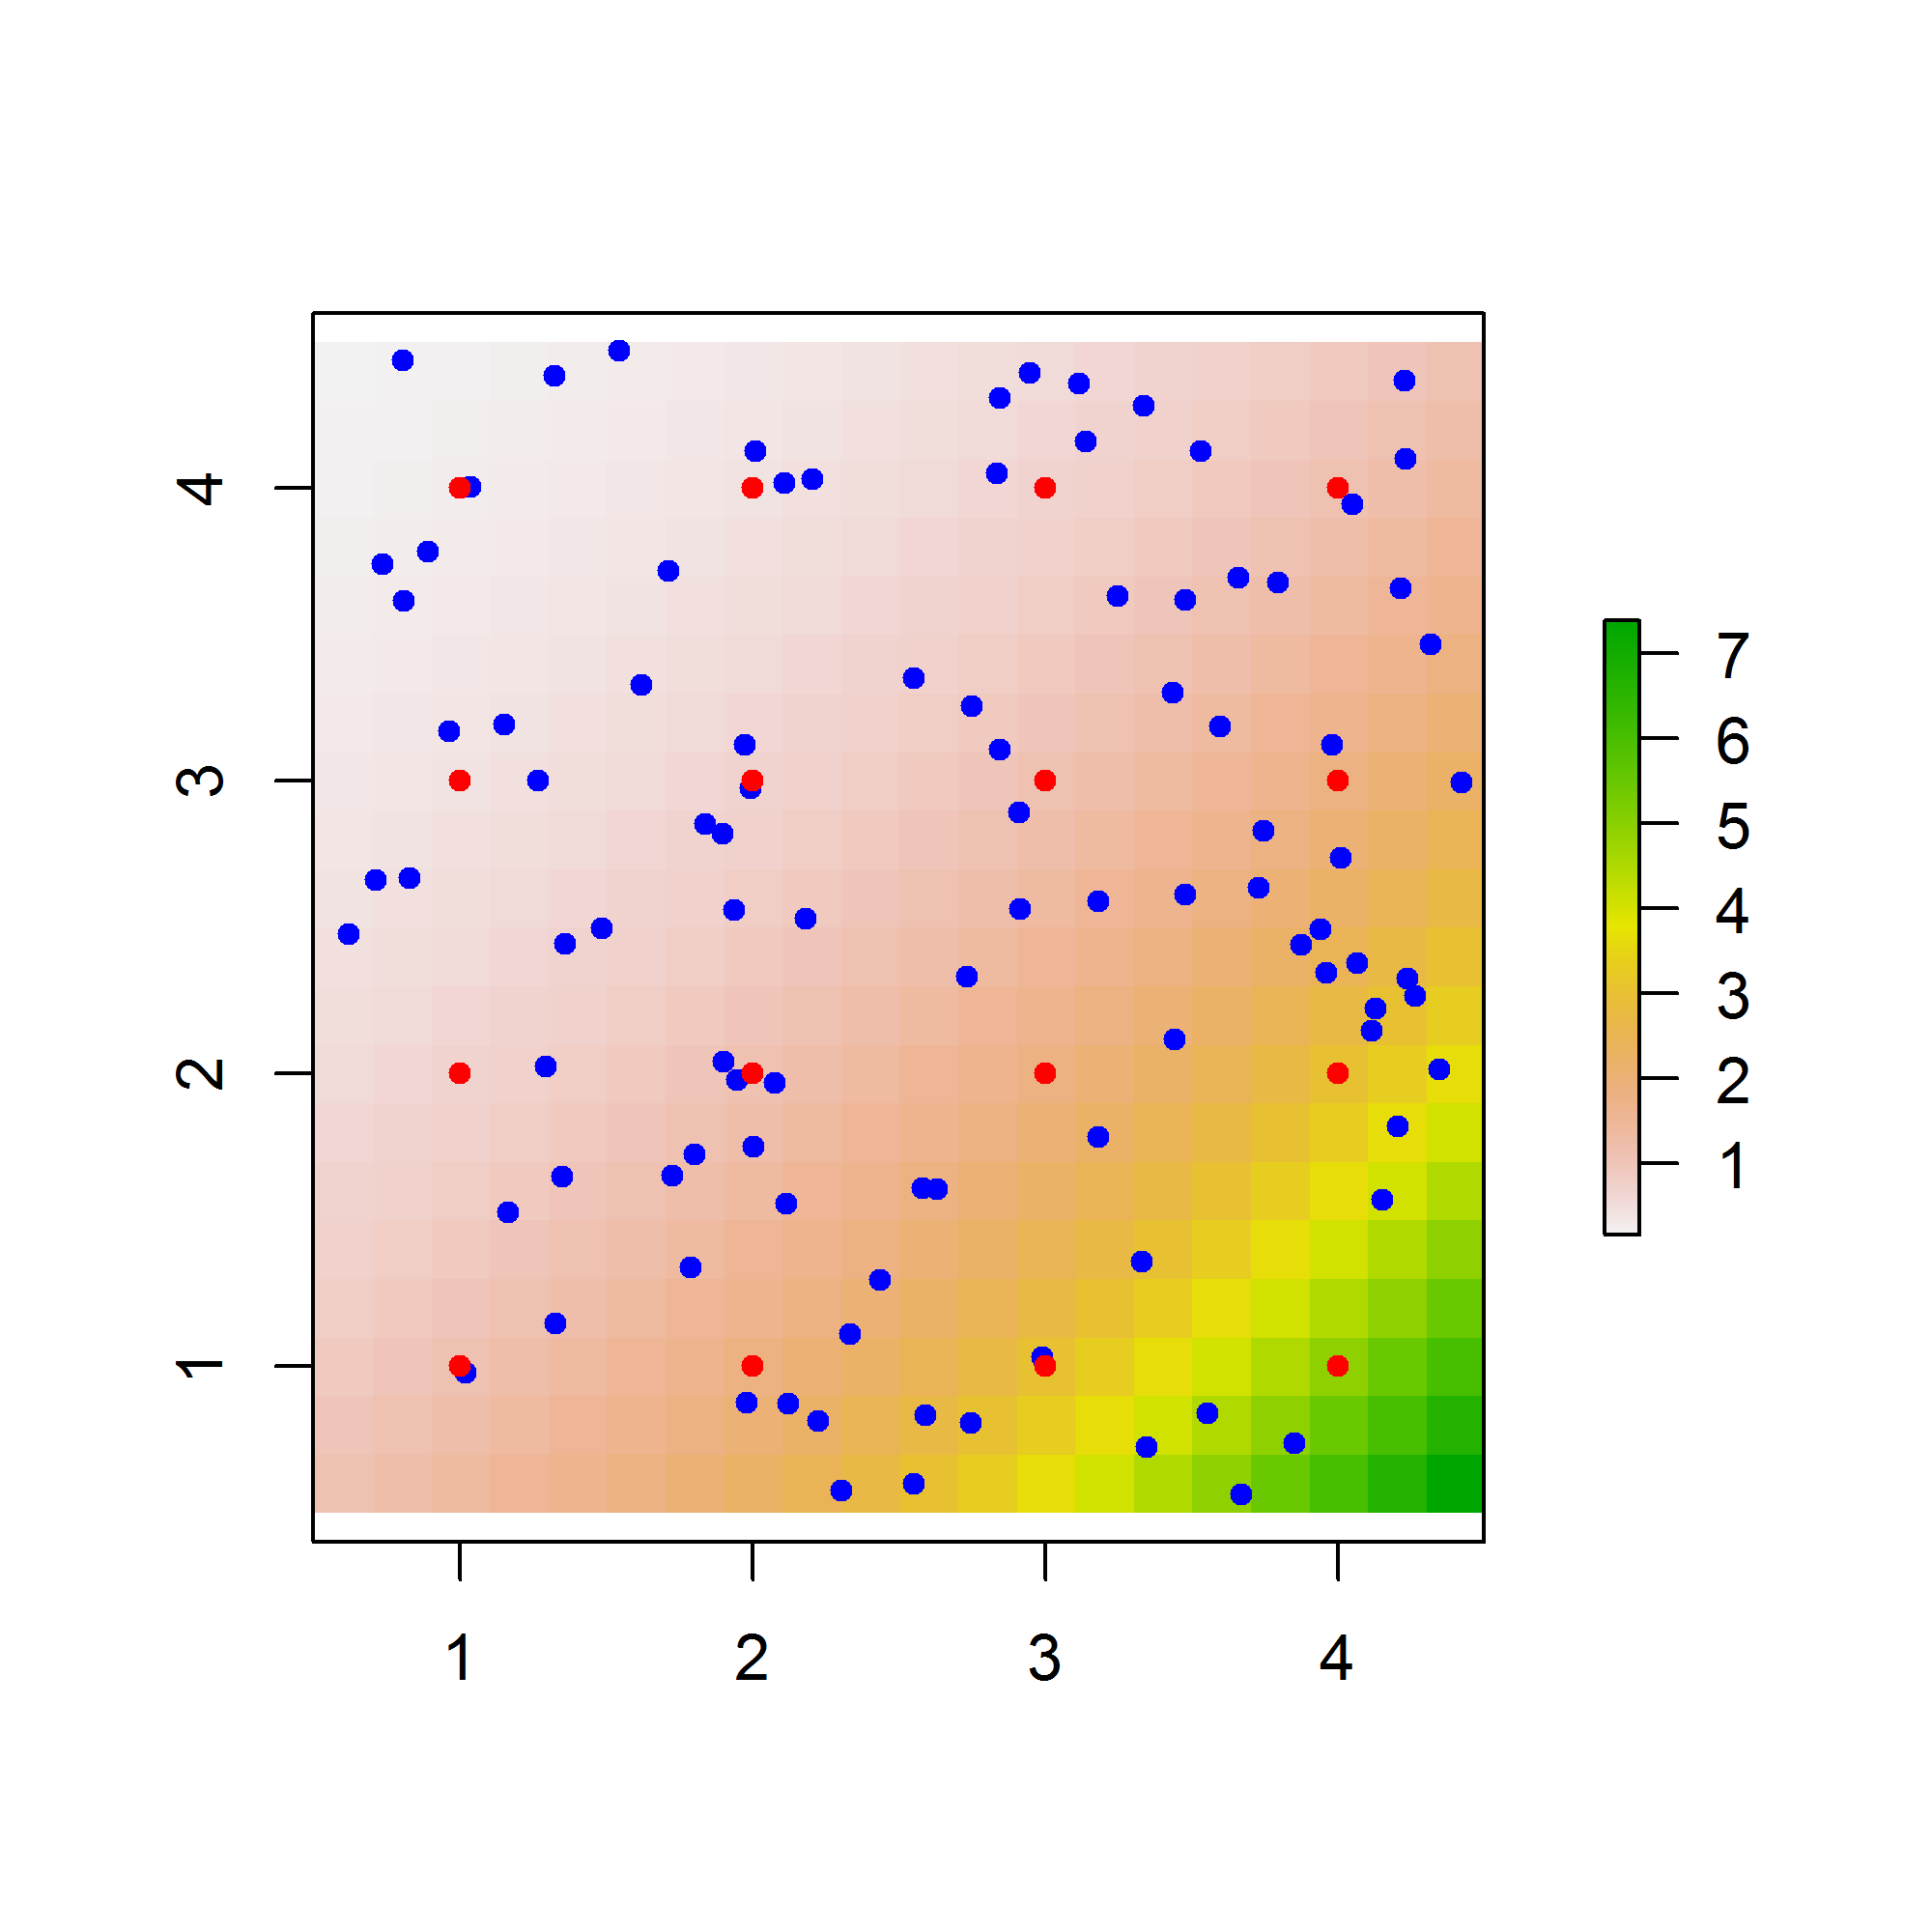
\includegraphics[height=3.25in,width=3.25in]{raster_withN100}
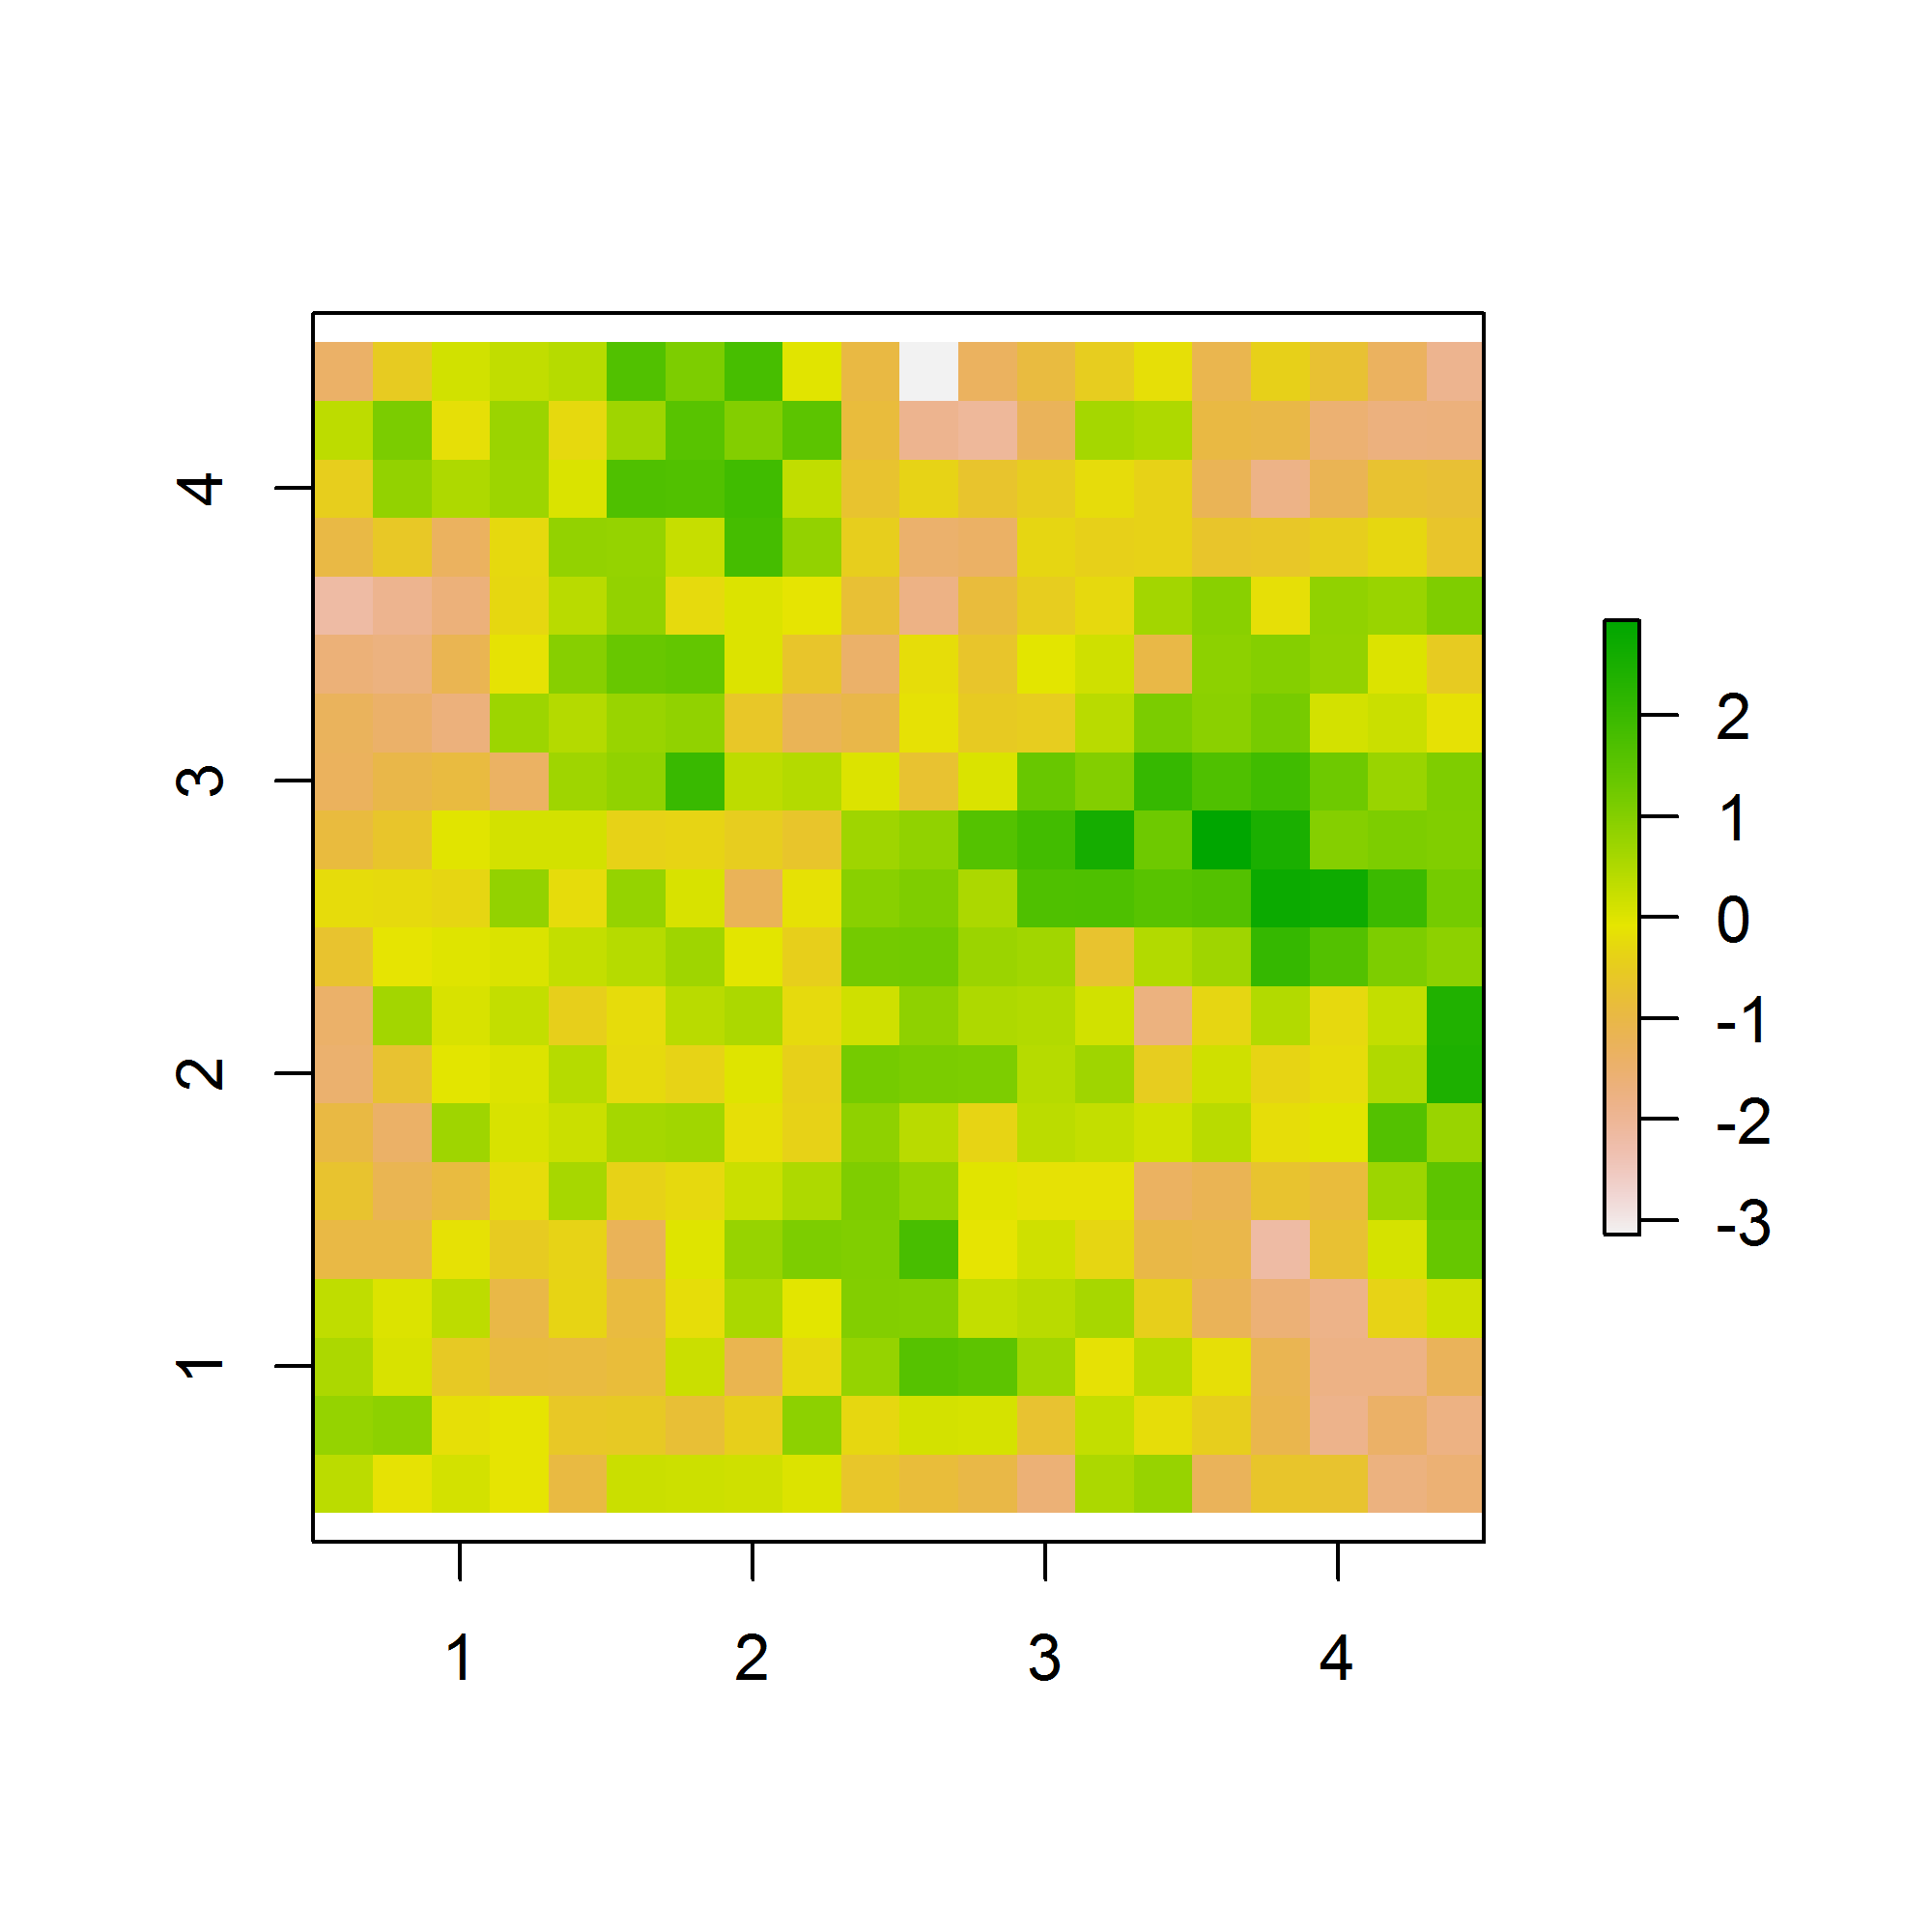
\includegraphics[height=3.25in,width=3.25in]{raster_krige} &
\end{tabular}
\caption{
Two landscape covariates used for simulations. A hypothetical
  realization of $N=100$ activity centers is superimposed on the left,
along with 16 trap locations.
}
\label{ecoldist.fig.raster100}
\end{figure}




\clearpage

\newpage




\end{document}






